\documentclass{article}

\usepackage{swiftnav}
\usepackage{pgfplots}
\usepackage{filecontents}

\usepackage{draftwatermark, array}
\SetWatermarkLightness{0.9}
\SetWatermarkText{Preliminary}
\SetWatermarkScale{1}
% Suppress numbers from section headings (but preserve PDF TOC).
\makeatletter
\renewcommand\@seccntformat[1]{}
\makeatother
\newcolumntype{$}{>{\global\let\currentrowstyle\relax}}
\newcolumntype{^}{>{\currentrowstyle}}
\newcommand{\rowstyle}[1]{\gdef\currentrowstyle{#1}%
  #1\ignorespaces
}
\newenvironment{mpar}{\par\noindent\minipage{\linewidth}}{\endminipage\par}
%\setlength{\skip\mpfootins}{2cm}
\renewcommand{\thempfootnote}{(\arabic{mpfootnote})}


% ---------------------------------------------------------------------------
\usepackage[section]{placeins}
\version{0.1}
\title{Piksi for UAV Aerial surveying}
\mysubtitle{RTK direct georeferencing with Swift Navigation's Piksi GPS receiver}
\author{Dennis Zollo, Rai Gohalwar}
\date{\today}

\ignorespaces

\begin{document}
\maketitle

\thispagestyle{firstpage}

\section{Abstract}
\label{sec:abstract}
This whitepaper presents using Piksi, a Carrier Phase differential GPS sensor, to georeference aerial images from micro aerial vehicles (MAVs) for surveying use cases.
It presents both the sensor integration, data collection methods, and real world surveying results as processed by the PIX4D photogrammetry software.  Lastly, the value proposition of using RTK GPS for aerial surveying is evaluated.
\tableofcontents
\newpage
\section{Overview}
\label{sec:Overview}
Due to the capability, low-cost, and popularity of micro aerial vehicles, there is much interest about their potential applications future applications. One promising application is aerial surveying for industries such as precision agriculture, mining, and forestry.

In a typical aerial surveying use-case, a fixed wing or multi-rotor aircraft is outfitted with a high-quality camera.  The vehicle overflies the area of interest and captures a series of images which are processed in software to produce Digital Elevation Models (DEM's), Orthomosaics, and/or 3D point clouds.  These models and deliverables, in turn, can be used for photogrammetry applications, volumetric measurements, or crop health measurements which can provide actionable business value for users.

Commercial software tools for photogrammetry have the ability to stitch together aerial images through visual features with techniques such as Bundle adjustment [TODO: Citations].  These software packages often require rough location and orientation of the lense when the photo was taken. To that end, most low-cost MAV control systems used for photogrammetry have the ability to geotag photos as required by the processing software. These vehicles often employ Autonomous or Single Point GPS combined with MEMS sensors to measure this information.  The typical sensor technology, combined with uncertainty in timing of the camera's shutter, limits the precision and accuracy of geotagging information and requires post-processing software to rely heavily on image processing techniques. Additionally, large amounts of sidelap and overlap between images and ground control points are often required to allow post-processing software to utilize imagery information given the inaccuracy of the georeferencing information.  Lastly, survey sites lacking in visual detail (such as agricultural land) or where overlap is minimal (such as corridor mapping), often yield poor results with traditional techniques and sensors.

It has been demonstrated that Carrier Phase Differential GPS (Also called Real Time Kinematic (RTK)), can improve the location accuracy of geo-referencing [Cite XBEE or other stuff here].  In the sections that follow, we will demonstrate methods and results of using Swift Navigation's Piksi GPS Receiver to geotag aerial photos for aerial surveying.  It is expected that precise and accurate geotagging information can reduce the need for ground control points for typical survey missions, reduce the amount of overlap and sidelap required, and improve the quality of ultimate photogrammetry deliverables.

\section{Equipment and Setup}
\label{sec:equipment}in
here we describe the equipment
\begin{figure}[h]
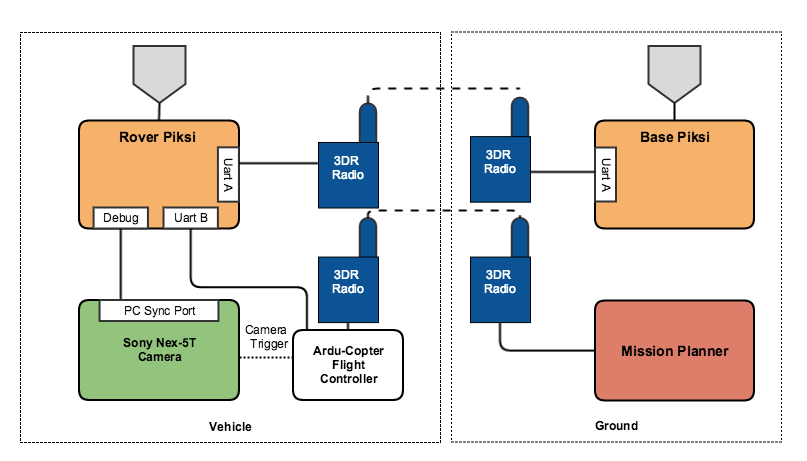
\includegraphics[width=7in]{images/flow_charts/uav_piksi_flow_chart.png}
\end{figure}

\begin{table}[]
\centering
\begin{tabular}{l ^ l}
\hline
\rowstyle{\bfseries}
Specification & Value \\ \hline
\rowstyle{}
Camera                                                                & Sony Nex-5T        \\ \hline
Lens                                                                  & Sony SEL-20F28 (20mm)     \\ \hline
\begin{tabular}[c]{@{}l@{}}Weight\\ (with vehicle mount)\end{tabular} & 424 g              \\ \hline
Sensor                                                                & 16 MP: 4912 x 3264 \\ \hline
Hot shoe adapter \begin{tabular}[c]{@{}l@{}}Fotasy SANEX Hot Shoe Adapter \\(ASIN: B00DE4T4E2)\end{tabular}  \\ \hline
\end{tabular}
\label{table:cameraspecs}
\caption{Camera Specifications}
\end{table}
\label{sec:equipment}
A camera, vehicle, and an image-tagging system using Piksi were developed to conduct experiments with careful design considerations.  Available and low cost COTS equipment was chosen to highlight that these results can be replicated without exotic or expensive equipment.  The camera chosen was a Sony NEX-5t with a fixed 20mm lense and a 16 MP CCID sensor.  The application required the ability to electrically sense the shutter which was achieved through the use of a "Fotasy SANEX Hot Shoe Adapter" Prontor/Compur (PC) socket for external flash Synchronization.  See table \ref{table:cameraspecs} for detailed camera specifications.

The vehicle was designed and sized to carry the camera payload for a typical surveying mission.  While a fixed wing aircraft may be more applicable to surveying missions for their increased range, a quadrotor configuration was chosen for low-cost and ease of implementation.  The test vehicle is based on a 680 Tarot quad frame and uses four TigerMotor antigravity 4006 motors with 15 inch propellers. The Pixhawk autopilot controls the aircraft and a 10.4Ah 6S battery pack powers. Fully loaded the copter has a flight time of about 30 minutes. The Sony camera is attached pointing down via a custom designed 3D printed a housing. See table \ref{table:vehicle-specs} for more information.
\begin{table}[]
\centering
\begin{tabular}{l^l}
\hline
\rowstyle{\bfseries}
Specification & Value \\ \hline
\rowstyle{}
Frame Type            & Quad-Rotor           \\ \hline
Frame                 & Tarot FY650          \\ \hline
Flight Controller     & 3DR Pixhawk          \\ \hline
Motors x 4            & T-Motor MN4006       \\ \hline
Motor Controllers x 4 & X-Rotor 40A OPTO     \\ \hline
Propellers x 4        & Tarot 1555 CF        \\ \hline
Batteries x 2         & Multistar 6S 5200mAh \\ \hline
Weight                & 2942 g               \\ \hline
\end{tabular}
\label{table:vehicle-specs}
\caption{Vehicle Specifications}
\end{table}

\begin{figure}[h]
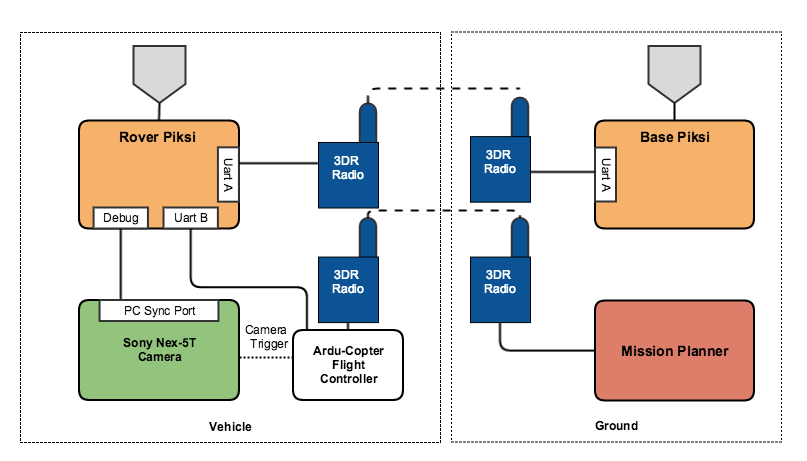
\includegraphics[width=7in]{images/flow_charts/uav_piksi_flow_chart.png}
\end{figure}


\begin{table}[]
\centering
\begin{tabular}{|l|c|}
\hline
\multicolumn{2}{|c|}{GPS Specifications} \\ \hline
Primary GPS         & Piksi v2.3.1       \\ \hline
Secondary GPS       & U-Blox NEO 7N      \\ \hline
Primary Antenna     & Tellysman TW2412   \\ \hline
Secondary Antenna   & Taoglas gp.1575    \\ \hline
\end{tabular}
\label{table:gps}
\caption{Vehicle GPS Specifications}
\end{table}
Camera, focal length, quadcopter
Radios
\section{Method}
\label{sec:method}
Site selection
GCP surveying (skylark)
Mission Planning (mission planner)
Camera setup (exposure, etc)
\section{Post-Processing Techniques}
\label{sec:epostprocessing}
Post processing tools were developed in house for this project. Images captures from the camera were not individually tagged. Instead , a file with the image names, Piksi geo-loacaiton data (WGS84) , orientation data (omega, phi, kappa) and accuracy (default of 5m horizontal and 10m vertical) was generated. This file was fed into Pix4D along with the images. Even though, 7 GCPs (Ground Control Points) were measure, none were used in the processing.

Figure 1 shows the basic layout of the post-processing setup.Georeference-process.py is a python scrypt that processes the data and generates a .csv file for Pix4d. There are other scryts within that carry out individual talks. Mavlink-decode.py extracts the piksi log file (SDBP JSON) from the dataflash BIN log file created by the Pixhawk. Interpolate-event.py linearly interpolates the position data at the trigger points using the SBP log file. Query-navlink.py is used to extract the attitude data at the trigger points. This attitude data is converted from centi-degrees to omega/phi/kappa in a subroutine in Georeference-process.py. All this data is then compiled into a file.


\begin{figure}
\begin{center}
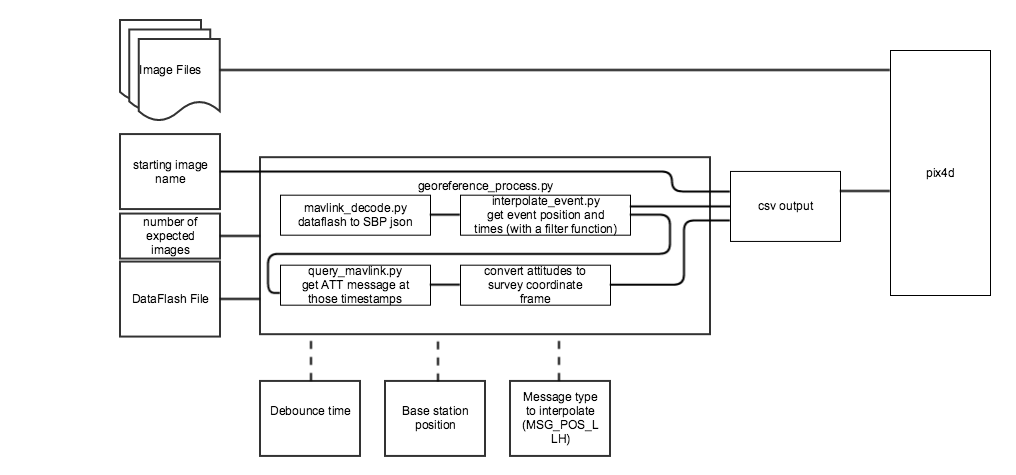
\includegraphics[width=7in]{images/flow_charts/uav_survey_processing_architecture.png}
\end{center}
\end{figure}

\begin{tabular}{l ^ l ^ l ^ l ^ l} \hline
\rowstyle{\bfseries}
Configuration & Description & Pix4D Calibration Method & GPS Sensor & Ground Control \\ \hline
\rowstyle{}
1 & Piksi RTK Std & All Images & Piksi RTK (Fixed) & No GCP \\ \hline
2 & Piksi RTK Std & Every Other Line & Piksi RTK (Fixed) & No GCP   \\ \hline
3 & Piksi RTK Std & Every Other Image & Piksi RTK (Fixed) & No GCP  \\ \hline
4 & Piksi RTK Std & All Images & Piksi RTK (Fixed) & GCP \\ \hline
5 & Piksi RTK Acc & All Images & Piksi RTK (Fixed) & No GCP \\ \hline
6 & Piksi RTK Acc & All Images & Piksi RTK (Fixed) & GCP \\ \hline
7 & Ublox Std & All Images & Ublox & No GCP   \\ \hline
8 & Ublox Std & Every Other Line & Ublox & No GCP \\ \hline
9 & Ublox Std & Every Other Image & Ublox & No GCP  \\ \hline
10 & Ublox Std & All Images & Ublox & GCP \\ \hline
11 & Ublox Acc & All Images & Ublox & No GCP \\ \hline
12 & Ublox Acc & All Images & Ublox & GCP \\ \hline
\end{tabular}
\section{Results: Accuracy}
talk about accuracy of each method

Accuracy is very important when conducting a surveying mission. Ideally GCPs help post-procesing softwares refine the scale and help allign the images better. Without GCPs , Pix4D would have a hard time computing the true scale of the image unless the geo-tags were really accurate. In order to test the accuracy of Piksi , we setup a test where we used Pix4D to measure the distance between 2 GCP markers. As shown in Figure ?? , these markers were red and white. Before the mission we collected the locations of these markers very accurately. Using some post-processing tools, we compared the calculated distances to the measured distance of 111111 metres. Results from this test are shown in table ?? . As the data shows, there is little to no difference between the distance Piksi renderings show compared to the ublox renderings. The hypothesis is that, if the data is within a threshold, Pix4D considers the geolocation data minutely. Most of the stitching and scaling is done from image processing.

\begin{tabular}{l ^ l ^ l ^ l ^ l} \hline
\rowstyle{\bfseries}
Configuration & X Error [m] & Y Error [m] & Z Error [m] & Images calibrated [percent]   \\ \hline
\rowstyle{}
1 & 0.185 & 0.136 & 0.274 & 84   \\ \hline
2 & 0.653 & 0.552 & 1.056 & 64    \\ \hline
3 & 0.847 & 1.182 & 1.202 & 59  \\ \hline
4 & 0.076 & 0.089 & 0.011 & 85    \\ \hline
5 & 0.556 & 0.619 & 0.989 & 99  \\ \hline
6 & 0.277 & 0.073 & 0.723 & 95   \\ \hline
7 & 0.202 & 0.840 & 0.563 & 82   \\ \hline
8 & 3.075 & 1.842 & 1.255 & 64   \\ \hline
9 & 2.191 & 3.028 & 1.897 & 57  \\ \hline
10 & 0.086 & 0.096 & 0.024 & 81   \\ \hline
11 & 0.500 & 0.625 & 0.959 & 99   \\ \hline
12 & WOULD & NOT & RENDER   \\ \hline
\end{tabular}

\begin{figure}
\begin{center}
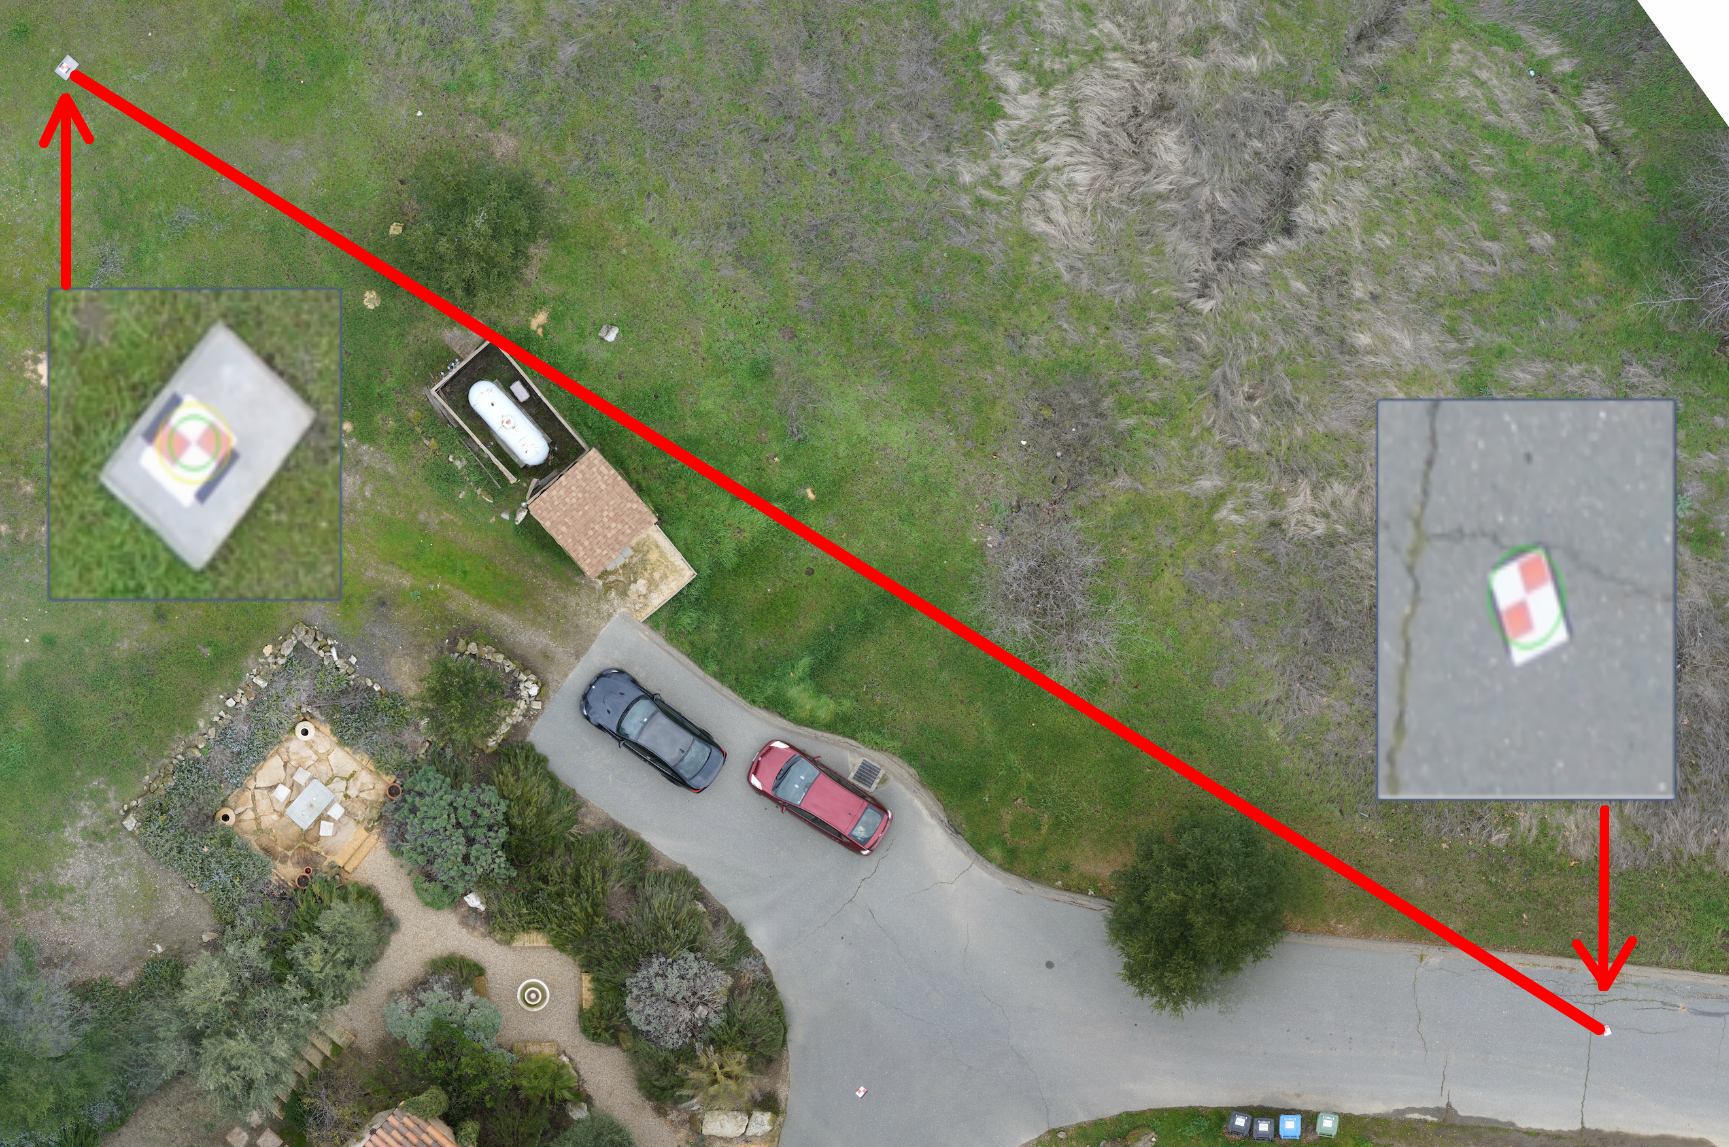
\includegraphics[width=5.5in]{images/accuracy_test_image.jpg}
\end{center}
\label{table:gps}
\caption{Vehicle GPS Specifications}
\end{figure}

\section{Results: Overlap/Sidelap}
Show that overlapp can be reduced with accurate geotag

The Survey mission was conducted with very high imagelap. With an overlap of 75 percent and a side lap of 60 percent, the mission was created so that in post processing we could eliminate lines and images and still be able to process the data. The average RMS error for XYZ was computed for all 6 configurations. Figure 1 shouws a graph of this data. Even though having a very small initial RMS error makes Piksi a clear winner over Ublox, Piksi also has a smaller magnitude of increased error. With every other line being processed, Piksi's errors went up 4.33 times and Ublox's errors went up 6.45 times. Moreover when every other image was processed, piksi's errors went up 5.89 times and Ublox's went up 6.65 times.
\begin{figure}
\begin{center}
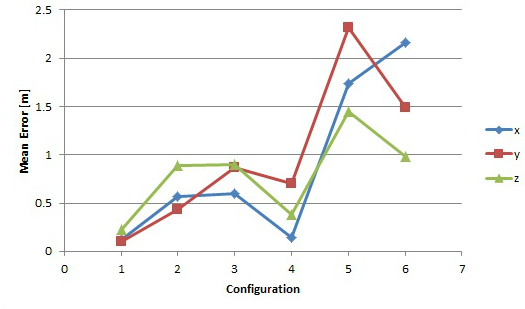
\includegraphics[width=5.5in]{images/rms_error_graph.jpg}
\end{center}
\label{table:gps}
\caption{Vehicle GPS Specifications}
\end{figure}

\section{Results: Initial accuracy estimate investigation}
One potential output to measure post-processing quality is the RMS errors reported by Pix4d Software which come from the "Initial processing" step of the software.  Indeed, the marketing material of some vendors and other parts of the literature use this image processing output as a key metric in evaluating the quality of geolocation surveying data.

In this analysis, however, the RMS errors values seemed highly affected by the image geolocation "accuracy" estimates are initially provided to the software by the user as input.  This outcome was peculiar and unexplained.  This odd relationship is presented in table [TABLE HERE]. The table shows three identical post-processing runs where the only difference was the accuracy estimate.  As this accuracy estimate decreased, the image location errors as reported in the Pix4d quality report decreased as well.  This behavior suggests that the accuracy reported by Pix4d for geolocation information is more an artifact of post-processing than representing something physical. As an additional note, in certain cases when these initial accuracy values are constrained to values below the accuracy of the sensors used for geo-referenceing, the software is unable to perform initial processing.

 % images processed  2d keypoints mean RMS Error [m] X RMS Error [m] Y RMS Error [m] Z
\begin{tabular}{l ^ l ^ l ^ l ^ l ^ l ^l ^l ^l ^l} \hline
\rowstyle{\bfseries}
Render label & Processing Time & Total Images & \multicolumn{2}{^l^}{Initial Image Accuracy [m]}  &  images processed & 2d keypoints & \multicolumn{3}{^l^}{Mean RMS Error [m]}
\rowstyle{}
a  & 1:46:58 &218 &5   &10  &84  &5902  &0.184857  &0.136434  &0.273608 \\ \hline
b  & 01:30:50&218 &0.2 &1   &84  &5907  &0.126739  &0.097678  &0.163582 \\ \hline
c  & 1:08:14 &218 &0.1 &0.2 &84  &5887  &0.061538  &0.06066   &0.111367 \\ \hline
\end{tabular}
\thispagestyle{lastpage}
\end{document}
